\documentclass[10pt, a4paper, italian]{article}
\usepackage[T1]{fontenc}
\usepackage[utf8]{inputenc}
\usepackage{amsmath, amssymb, amsthm, thmtools, amsfonts, mathtools}
\usepackage{nicefrac}
\usepackage{calc}
\usepackage[pdftex, hyperindex, plainpages=false]{hyperref}
\usepackage[nameinlink]{cleveref} %load before classicthesis (clash)
%\usepackage[nochapters,pdfspacing]{classicthesis}
\usepackage{siunitx}
\usepackage[siunitx]{circuitikz}

\usepackage[a4paper]{geometry}
\usepackage{float}
\usepackage{mdframed}
\usepackage{titling}
\usepackage{booktabs}
\usepackage{graphicx}
\usepackage{caption, subcaption}
\usepackage{xcolor}
\usepackage[italian]{babel}
\usepackage{pgfplots}
\usepackage{listings}
%\usepackage{lmodern}
\usepackage{url}
\usepackage{enumitem}
\usepackage{tikz} %loads after classicthesis (xcolor incompat)

% lets graphicx know path where figures to be included are found
\graphicspath{{../figs/}}
\makeatletter
\def\input@path{{../figs/}}
%or: \def\input@path{{/path/to/folder/}{/path/to/other/folder/}}
\makeatother

% tikz pgf plots setup
\usepgfplotslibrary{external}
\pgfplotsset{compat=1.15}
%\tikzexternalize

% spaces and significant digits/figures for measurements
\sisetup{free-standing-units, space-before-unit, number-unit-product = \;,
scientific-notation = false, round-mode = figures, round-precision = 1,}

% turns all (hyperlinked) references black [default is blue]
\hypersetup{
	linktoc=all,
	colorlinks=true,
	linkcolor=black
}

% code listings config
%\lstset{
%language=Python,
%basicstyle=\ttfamily,
%columns=fullflexible,
%keepspaces=true,
%}

% mdframed (for boxed text) configuration
\mdfsetup{linewidth=0.6pt}

% Default fixed font does not support bold face
\DeclareFixedFont{\ttb}{T1}{txtt}{bx}{n}{12} % for bold
\DeclareFixedFont{\ttm}{T1}{txtt}{m}{n}{12}  % for normal

% Custom colors
\usepackage{color}
\definecolor{deepblue}{rgb}{0,0,0.5}
\definecolor{deepred}{rgb}{0.6,0,0}
\definecolor{deepgreen}{rgb}{0,0.5,0}

% Commands 
\newcommand{\executeiffilenewer}[3]{%
	\ifnum\pdfstrcmp{\pdffilemoddate{#1}}%
		{\pdffilemoddate{#2}}>0%
	{\immediate\write18{#3}}\fi%
}
% input .svg --> .pdf_tex graphs
%\newcommand{\includesvg}[1]{%
%	\executeiffilenewer{#1.svg}{#1.pdf}%
%	{inkscape -z -D --file=#1.svg %
%	--export-pdf=#1.pdf --export-latex}%
%	\input{#1.pdf_tex}%
%}
% Thanks UniPi's Department of Physics E. Fermi
\newcommand{\thanksdf}{(\thanks{Dipartimento di Fisica E.~Fermi,%
Universit\`a di Pisa - Pisa, Italy.}\;)}

% hyperlink to email address
\newcommand{\mail}[1]{\href{mailto:#1}{\textsf{#1}}}

% \vec for bold vectors, instead of overarrows (now "\arrvec")
\let\arrvec=\vec
\renewcommand{\vec}[1]{\boldsymbol #1}
% replaces straight phi with slanted phi
\renewcommand{\phi}{\varphi}
% replaces straight eps with curved epsilon
\newcommand{\eps}{\varepsilon}
% abbreviation for (sub_/super^)scripts of \lim, \sum,... in inline math
\newcommand{\ds}{\displaystyle}

% blackboard/number set letters
\newcommand{\CC}{\mathbb C}
\newcommand{\HH}{\mathbb H}
\newcommand{\KK}{\mathbb K}
\newcommand{\NN}{\mathbb N}
\newcommand{\PP}{\mathbb P}
\newcommand{\QQ}{\mathbb Q}
\newcommand{\RR}{\mathbb R}
\newcommand{\ZZ}{\mathbb Z}

\newcommand{\Abs}[1]{{\left\Vert #1\right\Vert}}
\newcommand{\enclose}[1]{{\left( #1 \right)}}
\newcommand{\Enclose}[1]{{\left[ #1 \right]}}
\newcommand{\floor}[1]{\left\lfloor #1 \right\rfloor}
\newcommand{\ceil}[1]{\left\lceil #1 \right\rceil}
\newcommand{\To}{\rightrightarrows}

% Math operators
\DeclareMathOperator{\divergence}{div}
\renewcommand{\div}{\divergence}
\DeclareMathOperator{\Imaginarypart}{Im}
\renewcommand{\Im}{\Imaginarypart}
\DeclareMathOperator{\Realpart}{Re}
\renewcommand{\Re}{\Realpart}
%\DeclareMathOperator{\arg}{arg}
\DeclareMathOperator{\tg}{tg}
\DeclareMathOperator{\arctg}{arctg}
\DeclareMathOperator{\settsinh}{settsinh}
\DeclareMathOperator{\settcosh}{settcosh}
\DeclareMathOperator{\tr}{tr}
\DeclareMathOperator{\im}{im}
\DeclareMathOperator{\sgn}{sgn}
\DeclareMathOperator{\diag}{diag}

\DeclarePairedDelimiter{\norm}{\lVert}{\rVert}
\DeclarePairedDelimiter{\scalar}{\langle}{\rangle}

% Logarithm with arbitrary base.
% -> log_10
\newcommand{\llog}[1][10]{\log_{#1}}

% Absolute value.
% -> |x|
\newcommand{\abs}[1]{\left| #1 \right|}

% Powers.
% -> x^a
\newcommand{\power}[2][2]{\left( #2 \right)^{#1}}

% Square.
% -> x^2
\newcommand{\sq}[1]{\power[2]{#1}}

% Expansion of the binomial coefficient.
% -> n1!/(n2!(n1 - n2)!)
\newcommand{\binomexpr}[2]{\frac{#1!}{#2!(#1 - #2)!}}

% Expression evaluation at a given point with square brackets.
% -> [x]_{a}
\newcommand{\at}[2]{\left[ #1\right]_{\makebox[-1pt][l]{${\scriptstyle#2}$}}}

% Expression evaluation in an interval.
% -> [x] _{a}^{b}
\newcommand{\eval}[3]{\left.#1%
  \right|_{\makebox[-1pt][l]{${\scriptstyle#2}$}}^{\makebox[-1pt][l]{${\scriptstyle#3}$}}}

% Upright d in math mode (for differentials).
% -> d
\newcommand{\ud}{\mathrm{d}}

% Differential.
% -> dx
\newcommand{\diff}[1][x]{\,\ud{#1}}

% Base command for defining derivatives.
% -> df/dx or d^kf/dx^k
\newcommand{\basederivative}[4][]{%
  \displaystyle%
  \ifx\\#1\\\frac{#4#2}{#4#3}%
  \else%
  \frac{#4^#1#2}{#4#3^#1}%
  \fi%
}

% Total derivative.
% -> df/dx(x) or d^kf/dx^k(x)
\newcommand{\td}[4][]{%
  \basederivative[#1]{#2}{#3}{\ud}%
  \ifx\\#4\\%
  \else%
  \mkern-4mu\left(#4\right)%
  \fi%
}

% Partial derivative.
% -> df/dx(x) or d^kf/dx^k(x)
\newcommand{\pd}[4][]{%
  \basederivative[#1]{#2}{#3}{\partial}%
  \ifx\\#4\\%
  \else%
  \mkern-4mu\left(#4\right)%
  \fi%
}

\newcommand{\intinf}{\int_{-\infty}^{\infty}\!\!\!}

\newcommand{\cinterval}[2]{\left[\, #1,~#2 \,\right]}

\newcommand{\linterval}[2]{\left[\, #1,~#2 \,\right)}

\newcommand{\rinterval}[2]{\left(\, #1,~#2 \,\right]}

\newcommand{\ointerval}[2]{\left(\, #1,~#2 \,\right)}

\newcommand{\prob}[1]{\displaystyle P\left(#1\right)}

\newcommand{\pvalue}{\emph{$p$-value}}

\newcommand{\cond}{\,|\,}

\newcommand{\expect}[1]{\displaystyle E\left[#1\right]}

\newcommand{\mom}[2][]{\displaystyle {\cal M}_{#2}\ifx\\#1\\\else(#1)\fi}

\newcommand{\momalg}[1]{\displaystyle \lambda_{#1}}

\newcommand{\momcen}[1]{\displaystyle \mu_{#1}}

\newcommand{\skewness}{\displaystyle \gamma_1}

\newcommand{\kurtosis}{\displaystyle \gamma_2}

\newcommand{\charf}[1][x]{\phi_{#1}}

\newcommand{\momgenf}[1][x]{M_{#1}}

\newcommand{\fwhm}{{\scriptstyle \textsc{FWHM}}}

\newcommand{\hwhm}{{\scriptstyle \textsc{HWHM}}}

\newcommand{\median}{\mu_{\nicefrac{1}{2}}}

\newcommand{\var}[1]{\ensuremath{\text{Var}\left(#1\right)}}

\newcommand{\cov}[2]{\ensuremath{\text{Cov}\left(#1, #2\right)}}

\newcommand{\corr}[2]{\ensuremath{\text{Corr}\left(#1, #2\right)}}

\newcommand{\like}{\mathcal L}

\newcommand{\likelihood}[2][]{\like\ifx\\#2\\\else(#2\ifx\\#1\\\else;#1\fi)\fi}

\newcommand{\chisq}{\ensuremath{\chi^2}}

\newcommand{\chisquare}[2][]{\chisq\ifx\\#2\\\else(#2\ifx\\#1\\\else;#1\fi)\fi}

\newcommand{\loglikelihood}[2][]{\log\likelihood[#1]{#2}}

\newcommand{\pdf}[3][]{#2(#3\ifx\\#1\\\else;#1\fi)}

\newcommand{\binomialpdf}[2][]{\pdf[#1]{\mathcal B}{#2}}

\newcommand{\multinomialpdf}[2][]{\pdf[#1]{\mathcal M}{#2}}

\newcommand{\poissonpdf}[2][]{\pdf[#1]{\mathcal P}{#2}}

\newcommand{\uniformpdf}[2][]{\pdf[#1]{u}{#2}}

\newcommand{\exponentialpdf}[2][]{\pdf[#1]{\varepsilon}{#2}}

\newcommand{\gausspdf}[2][]{\pdf[#1]{N}{#2}}

\newcommand{\chisquarepdf}[2][]{\pdf[#1]{\wp}{#2}}

\newcommand{\cauchypdf}[2][]{\pdf[#1]{c}{#2}}

\newcommand{\erf}[1]{\ensuremath{\text{erf}\left(#1\right)}}

\newcommand{\dccases}[4][]{#2 \ifx\\#2\\\else=\fi %
  \begin{cases}
    \displaystyle #3 & \text{per variabili discrete}\\
    \displaystyle #4 & \text{per variabili continue}#1
  \end{cases}
}
% sub/super-scriptable for all symbol as math operator 
\newcommand\Scaleforall[1]{\vcenter{\hbox{\scalefont{#1}$\forall$}}}

\DeclareMathOperator*\forevery{%
  \vphantom\sum
  \mathchoice{\Scaleforall{2}}{\Scaleforall{1.4}}{\Scaleforall{1}}{\Scaleforall{0.75}}}
\geometry{left=2cm, right=2cm, top=2cm, bottom=2cm}

% indexes subsections with letters, sections with numbers (1.a, 1.b, ...)
\renewcommand{\thesubsection}{\thesection.\alph{subsection}}

% lets graphicx know path where figures to be included are found
\graphicspath{{../figs/}}

\author{Gruppo 1.AC \\ Matteo Rossi, Bernardo Tomelleri}
\title{Es05A: Applicazioni non-lineari di amplificatori operazionali}
\begin{document}
\date{\today}
\maketitle

\setcounter{section}{0}

\section*{Misura componenti dei circuiti}
\begin{table}[htbp]
\centering
\begin{tabular}{cccccc}
\toprule
Resistenze $[\si{\ohm}]$ & $R$ & $\sigma R$ & Capacità $[\si{n\F}]$ & $C$ &
$\sigma C$ \\
\midrule
\midrule
$R_1$	  	& 992 	& 8		& $C_1$ & 212	& 9 \\
$R_2$	  	& 992	& 8		& & & \\
$R_4$	  	& 991	& 8		& & & \\
$R_5$	  	& 9.96 k	& 0.08	k& & & \\
$R_6$	  	& 99.9 k	& 0.8	k& & & \\
$R_7$	  	& 9.96 k& 0.08	k	& & & \\
$R_8$	  	& 104.6	k& 8		k& & & \\
$R_9$	  	& 103.0	k& 0.8	k	& & & \\
$R_{10}$  	& 100.6	k& 8		k& & & \\
$R_{11}$  	& 1.911	& 8		& & & \\
\bottomrule     
\end{tabular}
\caption{Valori di resistenza e capacità misurate per i componenti dei
circuiti studiati. \label{tab: rcmes_B}}

\begin{tabular}{cccccc}
\toprule
Resistenze $[\si{\ohm}]$ & $R$ & $\sigma R$ & Capacità $[\si{n\F}]$ & $C$ &
$\sigma C$ \\
\midrule
\midrule
$R_1$	  	& 996 	& 8		& $C_1$ & 207	& 9 \\
$R_2$	  	& 994	& 8		& & & \\
$R_4$	  	& 999	& 8		& & & \\
$R_5$	  	& 9.95	k& 0.08	k& & & \\
$R_6$	  	& 99.1	k& 0.8	k& & & \\
$R_7$	  	& 9.96	k& 0.08		k& & & \\
$R_8$	  	& 99.6	k& 0.8		k& & & \\
$R_{10}$  	& 99.8	k& 0.8		k& & & \\
$Pot_{R_9}$ & 103.4 k & 0.8 k& & & \\
$Pot_{R_11}$& 1.99 k & 0.08 k& & &\\
\bottomrule   
\end{tabular}
\caption{Valori di resistenza e capacità misurate per i componenti dei
circuiti studiati. \label{tab: rcmes_M}}
\end{table}

Riportiamo per completezza anche i valori delle tensioni di alimentazione
continue per l'op-amp misurate con il multimetro
\begin{align*}
V_{CC} &= 4.99 \pm 0.03 \si{\V} \\
V_{EE} &= -4.99 \pm 0.03 \si{\V}
\end{align*}


\subsection*{Nota sul metodo di fit}
Per determinare i parametri ottimali e le rispettive covarianze si \`e
implementato in \verb+Python+ un algoritmo di fit basato sui minimi quadrati
mediante la funzione \emph{curve\_fit} della libreria \texttt{SciPy}.

%=======================
\section{Generatore di Noise}
Il primo passo per la costruzione del circuito P.I.D. è la realizzazione del circuito di lettura. Nel nostro caso abbiamo realizzato un sistema di rilevazione di intensità luminosa basato su due circuiti per identici per emissione di luce (uno per il disturbo e l'altro di controllo) e un partitore di tensione costruito tramite una resistenza e una fotoresistenza.
\begin{figure}[H]
    \centering
	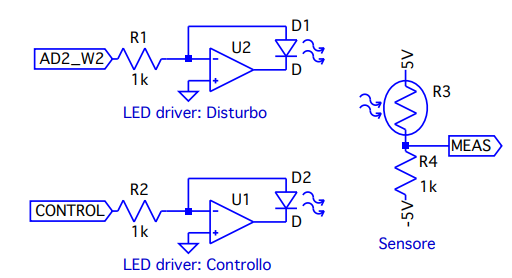
\includegraphics[scale=0.3]{noisegen}
    \caption{Schema circuitale per emissione e rilevazione intensità luminosa.
    \label{fig: Draft1}}
\end{figure}
\subsection{Funzionamento}
La fororesistenza è una resistenza variabile, che cambia col valore dell'intensità luminosa che incide su di essa, in particolare sappiamo che resistenza e quantità di luce sono inversamente proporzionali: maggiore sarà la luce incidente sulla superficie, minore sarà la sua resistenza.
Sappiamo dalla formula del partitore di tensione che il il valore dell'uscita MEAS sarà uguale a
\begin{equation}
V_{meas}=(V_{CC}- V_{EE})\frac{R_4}{R_4 + R_3}  + V_{EE}
\end{equation}
Ci aspettiamo quindi che aumentando la luce (per esempio nel nostro caso pilotando l'ingresso del LED driver di disturbo con una rampa), il valore di $V_{meas}$ andrà ad aumentare di conseguenza sempre nell'intervallo prefissato $(V_{EE},V_{CC})$.
Si è quindi presa una serie di misure di $V_{meas}$ per valori di tensione continua diversi all'entrata $AD2_{W2}$.
\begin{table}[H]
\centering
\begin{tabular}{@{}ll@{}}
\toprule
$V_{AD2_{W2}} [\si{\V}]$ & $V_{meas} [\si{\V}]$\\
\midrule
$-4.2 \pm 0.3$ m 	& $ -4.99 \pm 0.05$	\\
$995 \pm 7$ m 	& $ -2.11 \pm 0.02 $	\\
$1.99 \pm 0.02$ 	& $ -1.01 \pm 0.08 $\\
$2.98 \pm 0.04$ 	& $ -359 \pm 3 $ m\\
$3.98 \pm 0.04$ 	& $ 42.1 \pm 0.7 $ m\\
$4.98 \pm 0.05$ 	& $ 335 \pm 3$ m\\

\bottomrule
\end{tabular}
\caption{Misura di $V_{meas}$ in funzione della tensione in ingresso nel LED driver di disturbo}
\end{table}
Come ci aspettavamo il valore di $V_{meas}$ cresce aumentando la luce incidente, nel nostro caso, aumentando la tensione in ingresso $V_{AD2_{W2}}$.
%=======================
\section{Amplificatore del Noise rispetto al Set}
Si è costruito un amplificatore differenziale con guadagno $\approx 10$ a partire dalle resistenze $R_5$,$R_6$ e $R_7$,$R_8$ secondo lo schema in figura .
\begin{figure}[H]
    \centering
	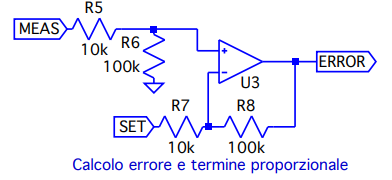
\includegraphics[scale=0.7]{errorgen}
    \caption{Schema circuitale per l'amplificatore differenziale 
    \label{fig: Draft1}}
\end{figure}
Lo scopo del circuito in figura è quello di amplificare la differenza tra i segnali $V_{set}$ e $V_{meas}$ di un fattore 10.
Si è quindi provato il guadagno per entrambi gli ingressi, inviando un segnale a uno e mettendo l'altro a massa; ci si aspetta che nel caso in cui set sia collegato al segnale in ingresso, l'uscita deve essere invertita, invece nell'altro caso meas e error devono essere in fase.
\begin{figure}[H]
    \centering
	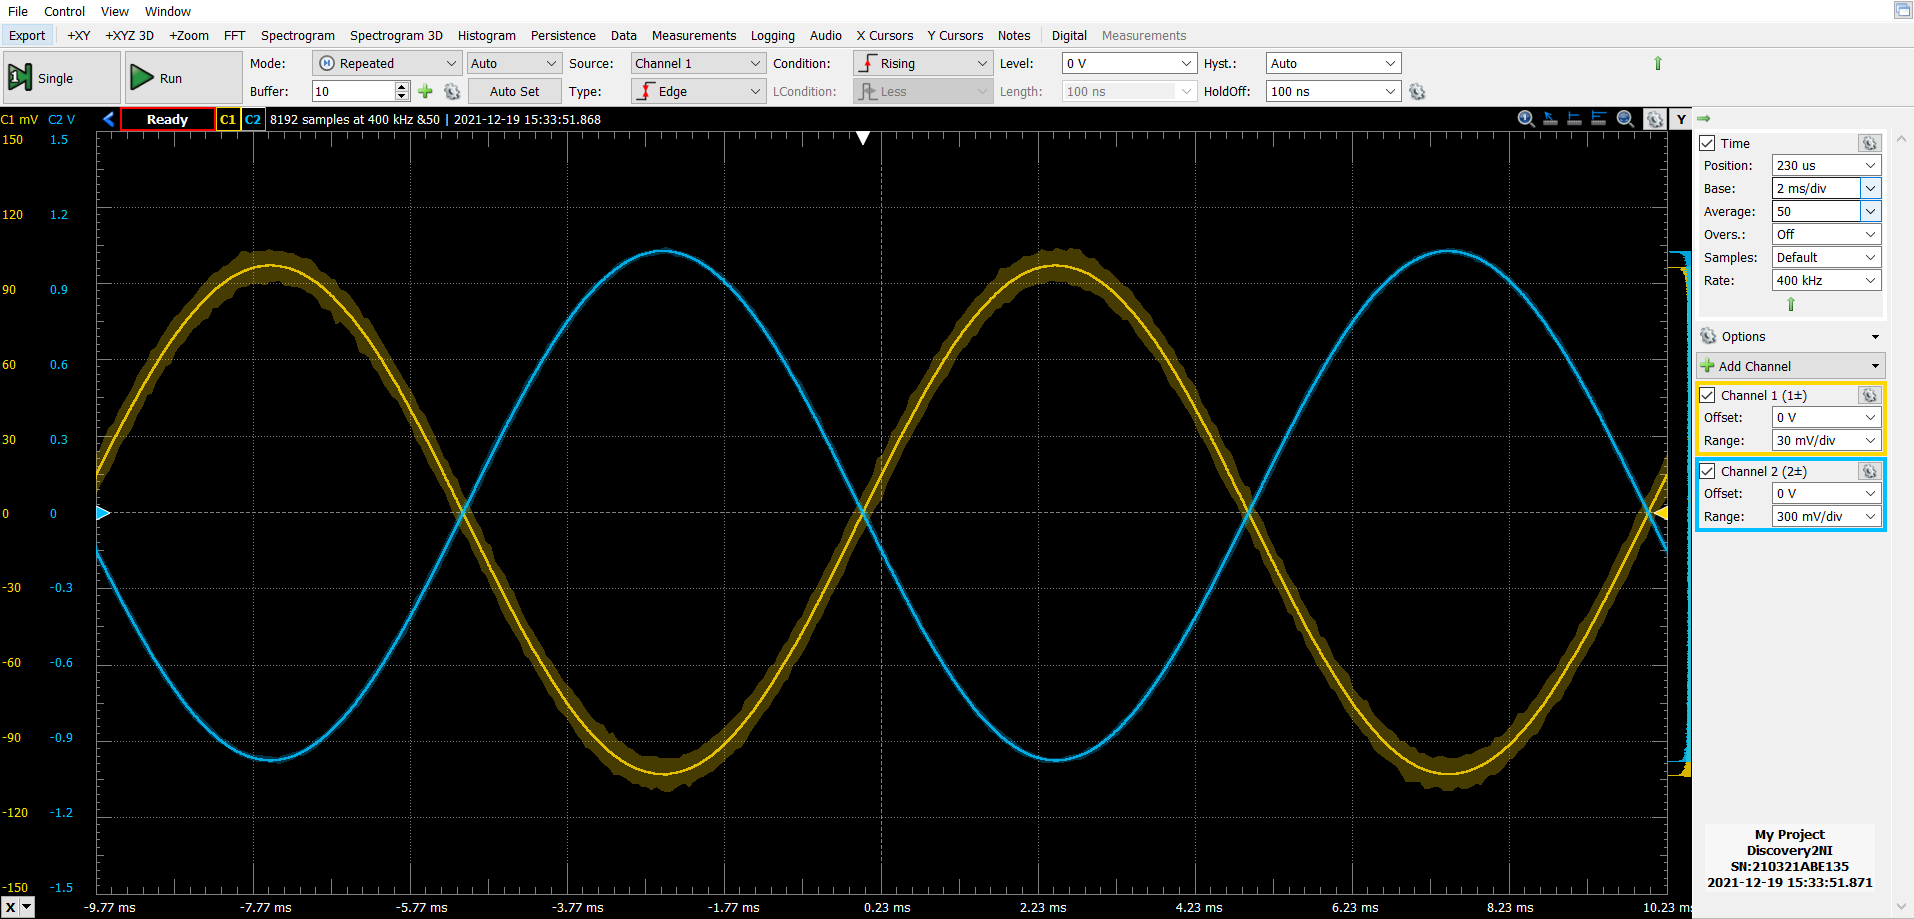
\includegraphics[scale=0.7]{error.set}
    \caption{Segnali in ingresso e uscita per l'amplificatore differenziale con meas collegato a massa: in giallo il canale Set, in blu il canale error.
    \label{fig: Draft1}}
\end{figure}
\begin{figure}[H]
    \centering
	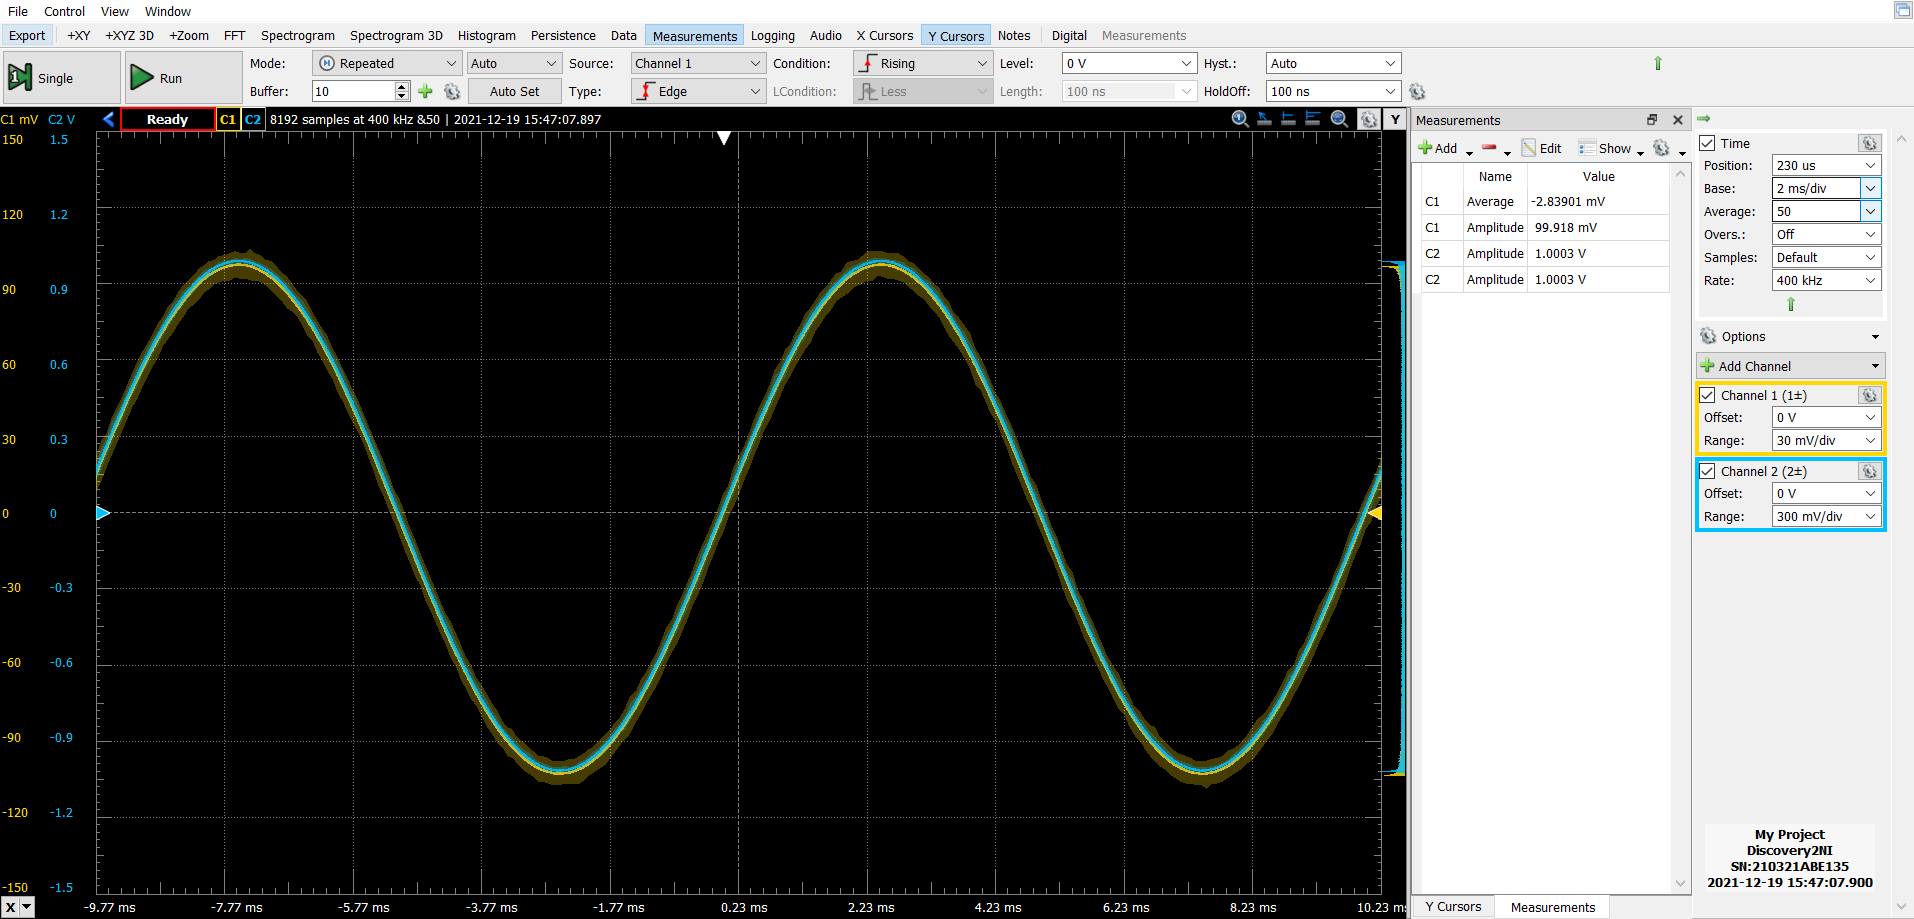
\includegraphics[scale=0.7]{error.meas}
    \caption{Segnali in ingresso e uscita per l'amplificatore differenziale con set collegato a massa: in giallo il canale Meas, in blu il canale error.
    \label{fig: Draft1}}
\end{figure}
Abbiamo quindi calcolato il guadagno come $A = \frac{V_{error}}{V_{signal}}$, che dà come risultato
\[
A=-10.01 \pm 0.14 
\]
\[
A=10.01 \pm 0.14
\]
per set e meas rispettivamente.\\
Per controllare la tensione di riferimento si è poi costruito un circuito che permettesse di variare $V_{set}$ nel solito intervallo $(V_{EE},V_{CC})$, per farlo abbiamo utilizzato un potenziometro da $2 k\ohm$.
\begin{figure}[H]
    \centering
	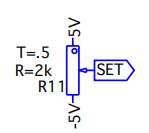
\includegraphics[scale=0.7]{setgen}
    \caption{Schema circuitale per la configurazione  della tensione del segnale di riferimento 
    \label{fig: Draft1}}
\end{figure}
Chiaramente essendo un amplificatore di differenza tra 2 segnali, nel caso in cui meas e set siano uguali $\implies$ la differenza è nulla $\implies V_{error} = 0$. Difatti utilizzando il canale uno per misurare il segnale meas rispetto al segnale set (per registrare la differenza tra i due segnali), e il canale 2 a misurare error rispetto a massa si registra quanto aspettato
\begin{figure}[H]
    \centering
	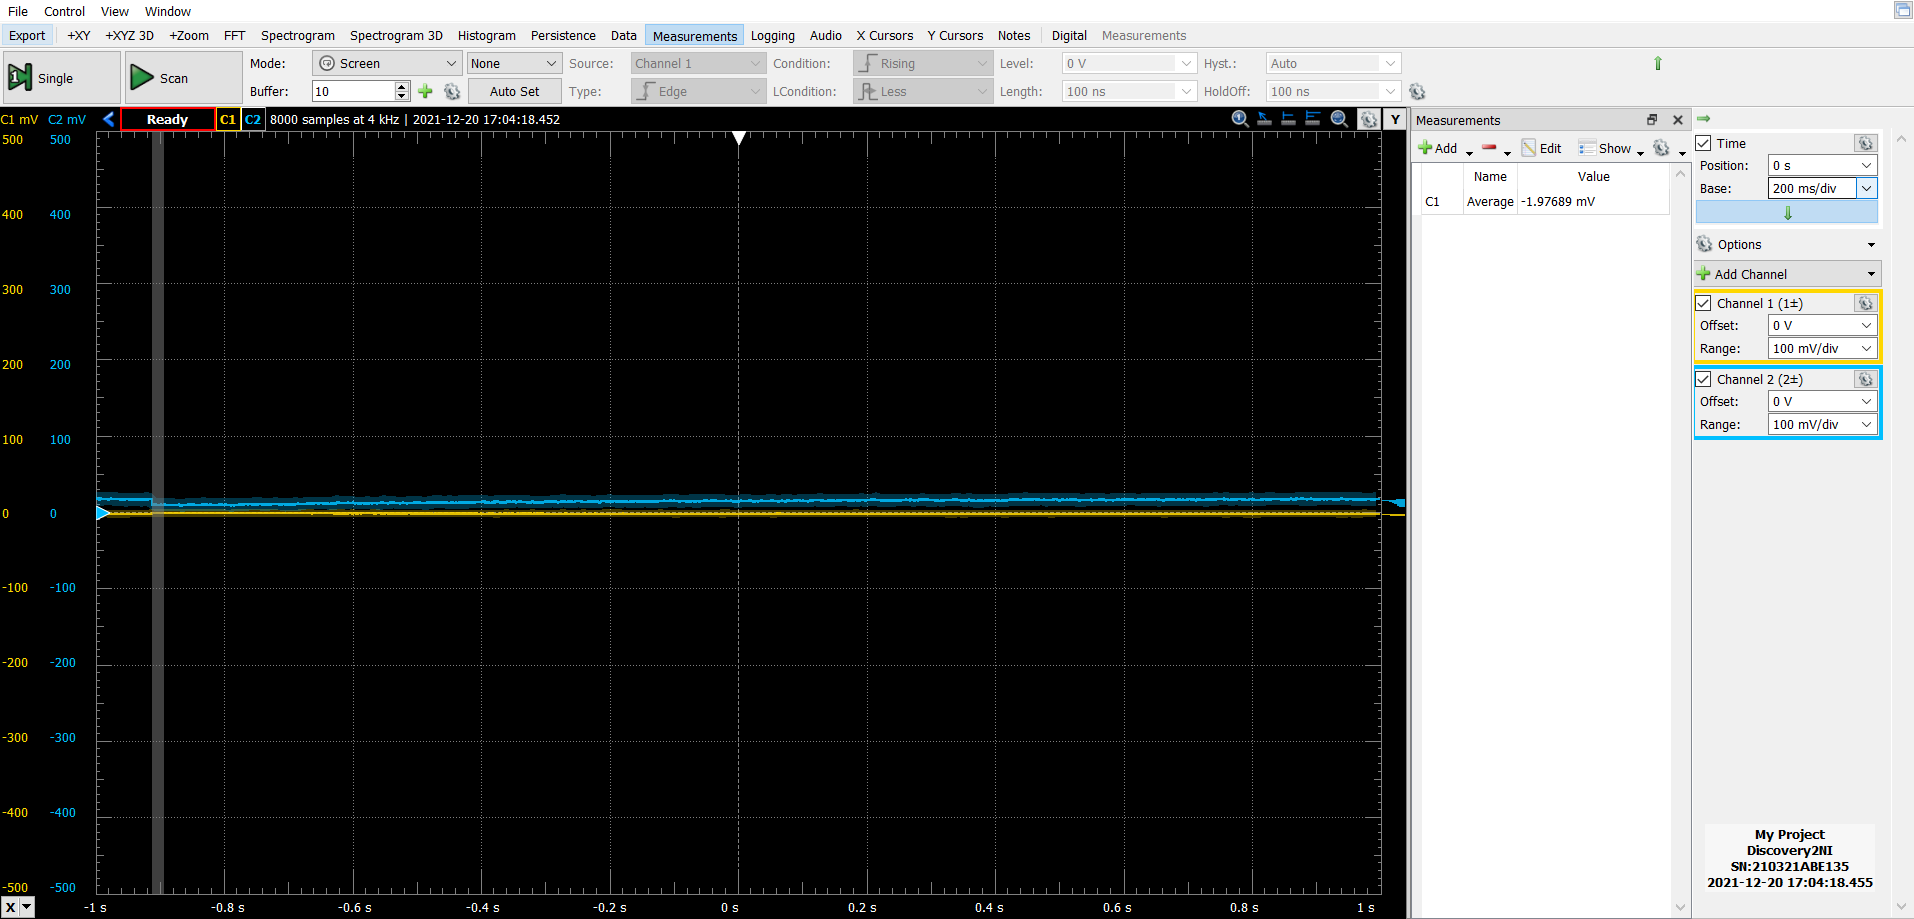
\includegraphics[scale=0.7]{meas.same.set}
    \caption{segnali nella condizione in cui il valore di set e meas sono uguali, nel canale uno si misura il valore di meas rispetto a set, nel canale due invece error rispetto a massa.
    \label{fig: Draft1}}
\end{figure}
%=======================
\section{Controllo integrale}
Successivamente si è montato il circuito di controllo integrale, un semplice circuito integratore, utilizzando la resistenza data dal potenziometro e una capacità $C_1$, utilizzando lo schema in figura
\begin{figure}[H]
    \centering
	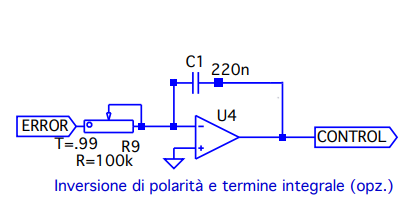
\includegraphics[scale=0.7]{controlgenint}
    \caption{schema circuitale del controllore ad azione integrale.
    \label{fig: Draft1}}
\end{figure}
quindi abbiamo collegato l'uscita control al driver per la luce di controllo e l'uscita del circuito di generazione errore all'entrata del circuito di controllo integrale.
Arrivati a questo punto è bastato spegnere il generatore di luce di disturbo e cambiare la posizione del potenziometro per permettere la led di controllo di accendersi.
Si nota subito come la risposta del led di controllo sia fortemente influenzata dalla quantità di luce che arriva alla fotoresistenza; si consiglia infatti di spostare il circuito distante da eventuali sorgenti di disturbo casuali, come per esempio persone che camminano in prossimità della fotoresistenza. 
Dopodiché si è provato a verificare la risposta del led di controllo ad un intervento esterno di riduzione della luce, abbiamo quindi posizionato delle buste di plastica semitrasparenti tra il diodo e la fotoresistenza: di conseguenza il led ha aumentato l'intensità luminosa.
\subsection{Risposta ad un'onda quadra}
Si è quindi passati alla verifica della risposta ad una luce di disturbo, in questo caso pilotata da un'onda quadra compresa tra 0 e 150 mV.
Per cominciare si deve fissare il valore di riferimento set: per farlo è bastato scegliere un'intensità luminosa casuale, per esempio quella che meas viene a registrare quando uno dei 2 driver led è pilotato con una tensione di 1 Volt, e utilizzare il potenziometro R11 per far combaciare i valori in meas e set.
A questo punto abbiamo inviato al led driver di disturbo un'onda quadra tra 0 e 150 mV con frequenza pari a 1 Hz.
Osservando il valore di control e meas ci rendiamo conto di quello che fa effettivamente il circuito, ovvero cerca di mantenere il valore di meas costante nel tempo.
\begin{figure}[H]
    \centering
	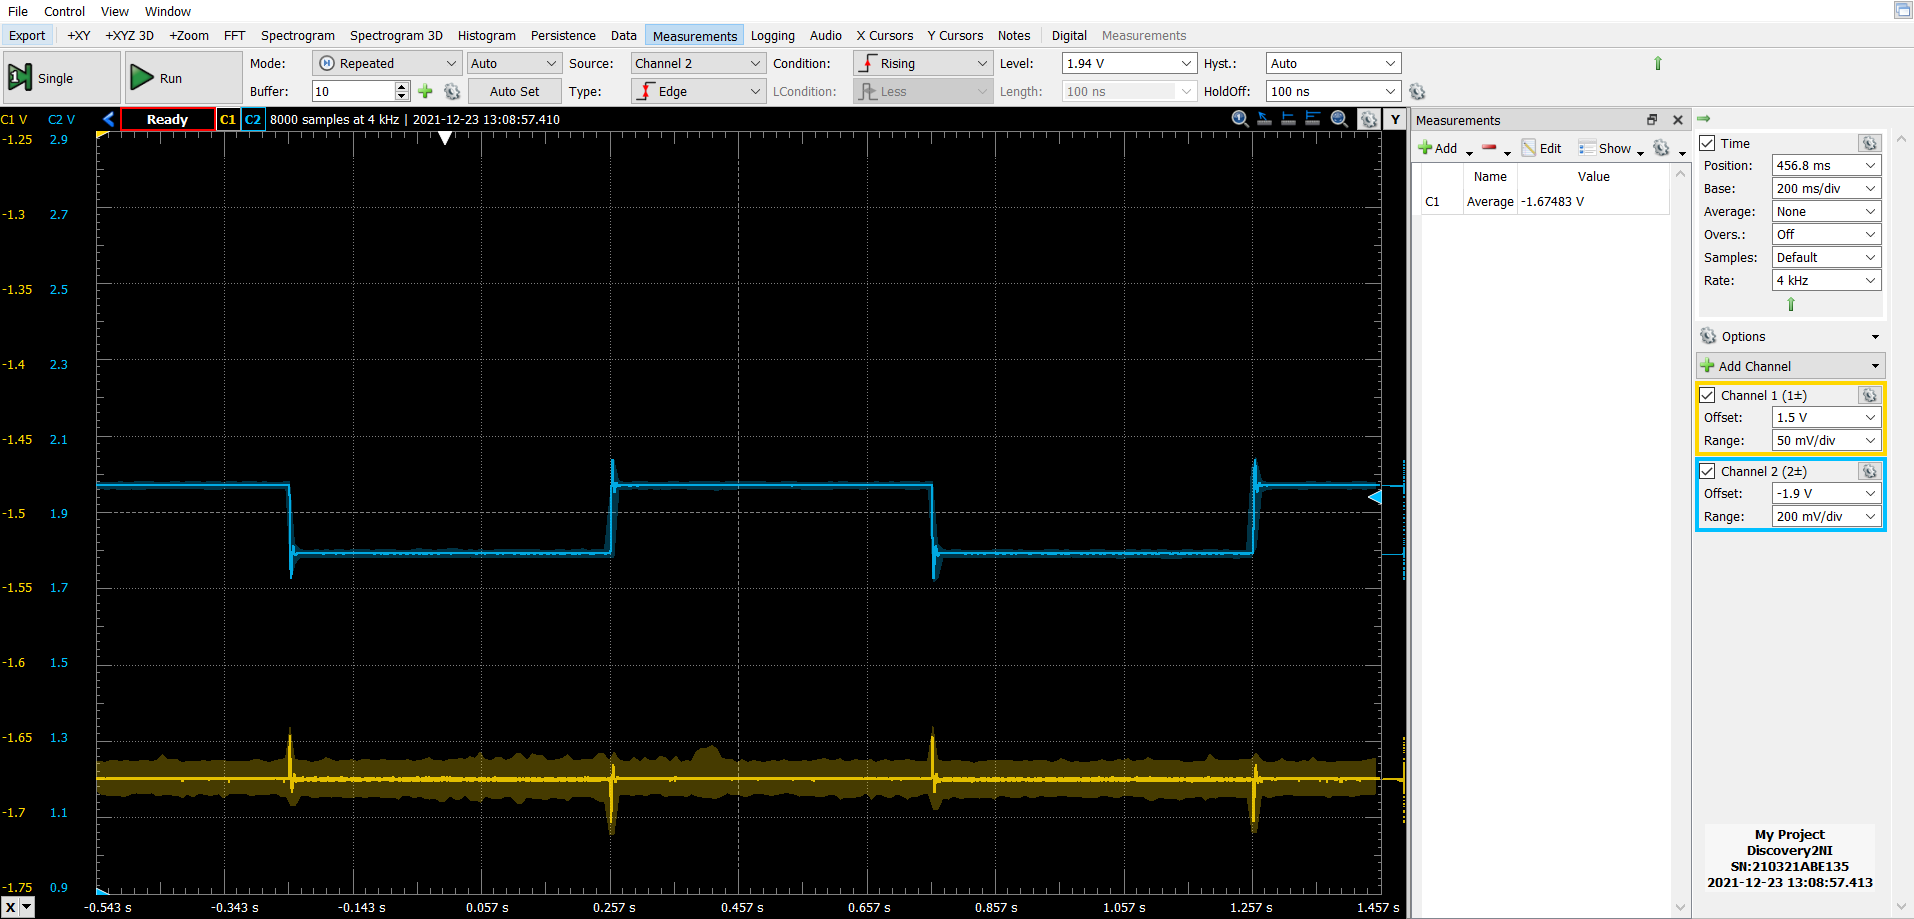
\includegraphics[scale=0.7]{control7.meas}
    \caption{grafico degli andamenti di control (rispetto a massa) in blu e di meas (sempre rispetto a massa) in giallo
    \label{fig: Draft1}}
\end{figure}
\begin{figure}[H]
    \centering
	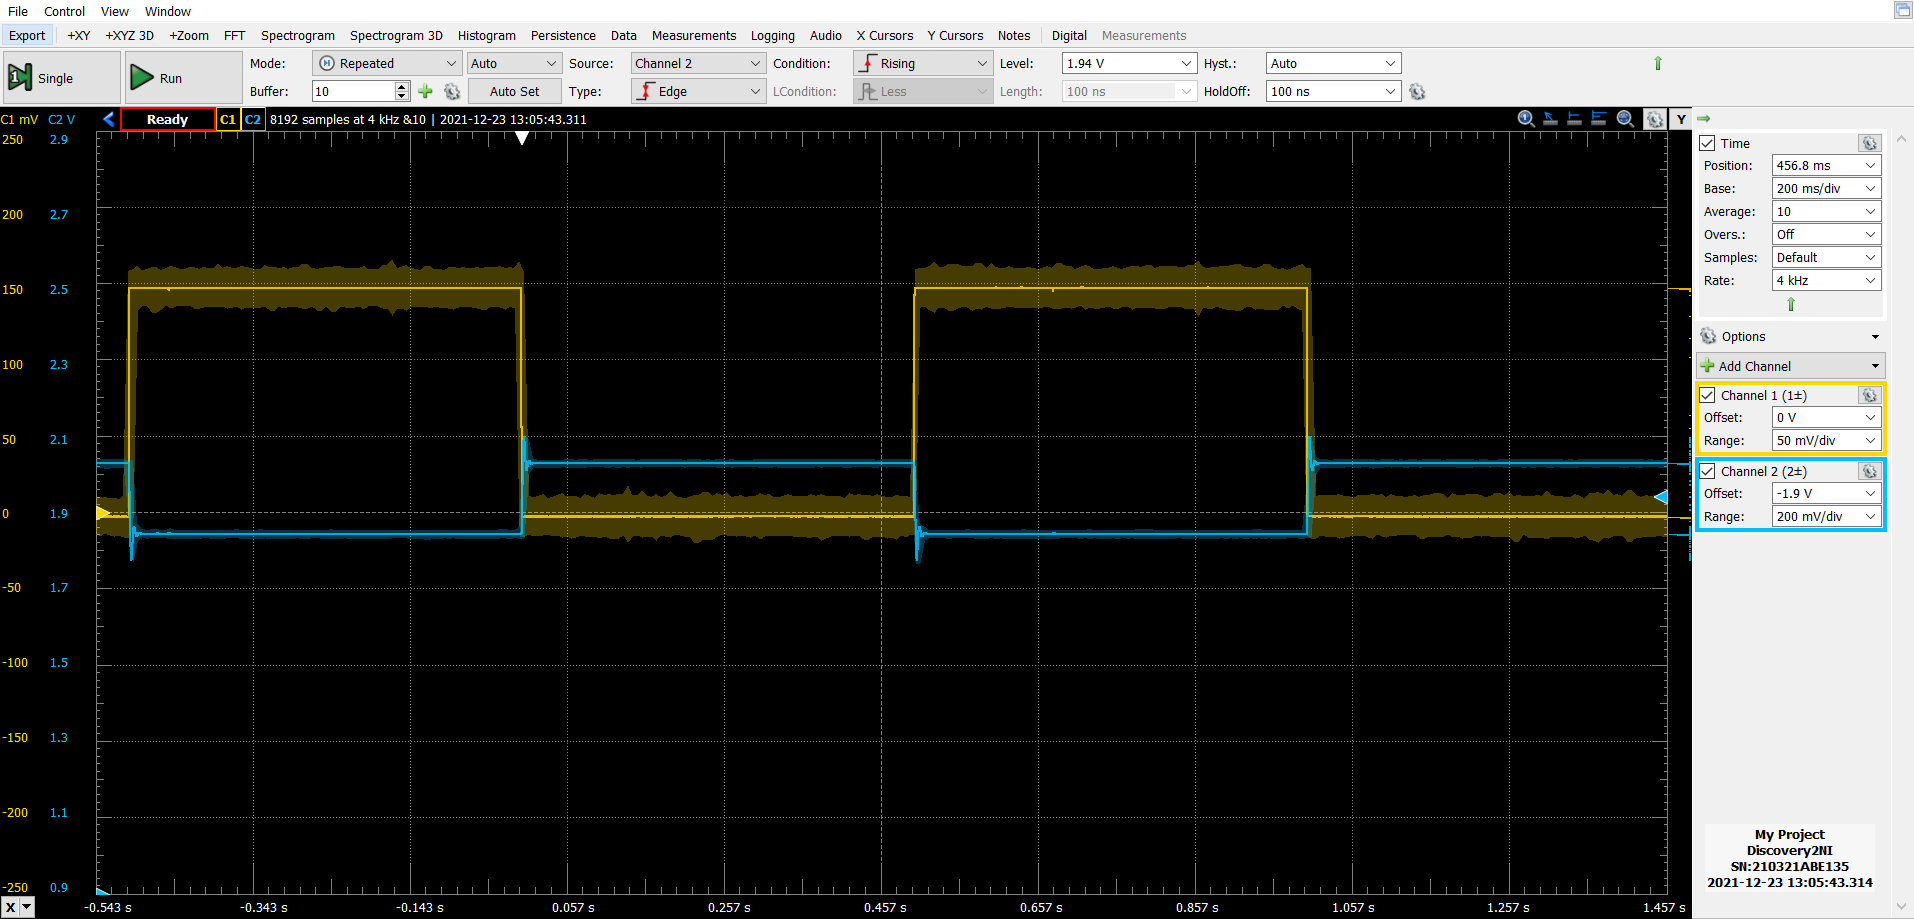
\includegraphics[scale=0.7]{control7}
    \caption{grafico del segnale control in blu e dell'onda pilota del led di disturbo in giallo
    \label{fig: Draft1}}
\end{figure}
Successivamente abbiamo misurato il canale error rispetto a massa per varie posizioni del potenziometro. In generale il segnale del canale error ha un andamento simile per ogni posizione, cambiano soltanto i tempi in cui il segnale torna ad essere 0.
\begin{figure}[H]
    \centering
	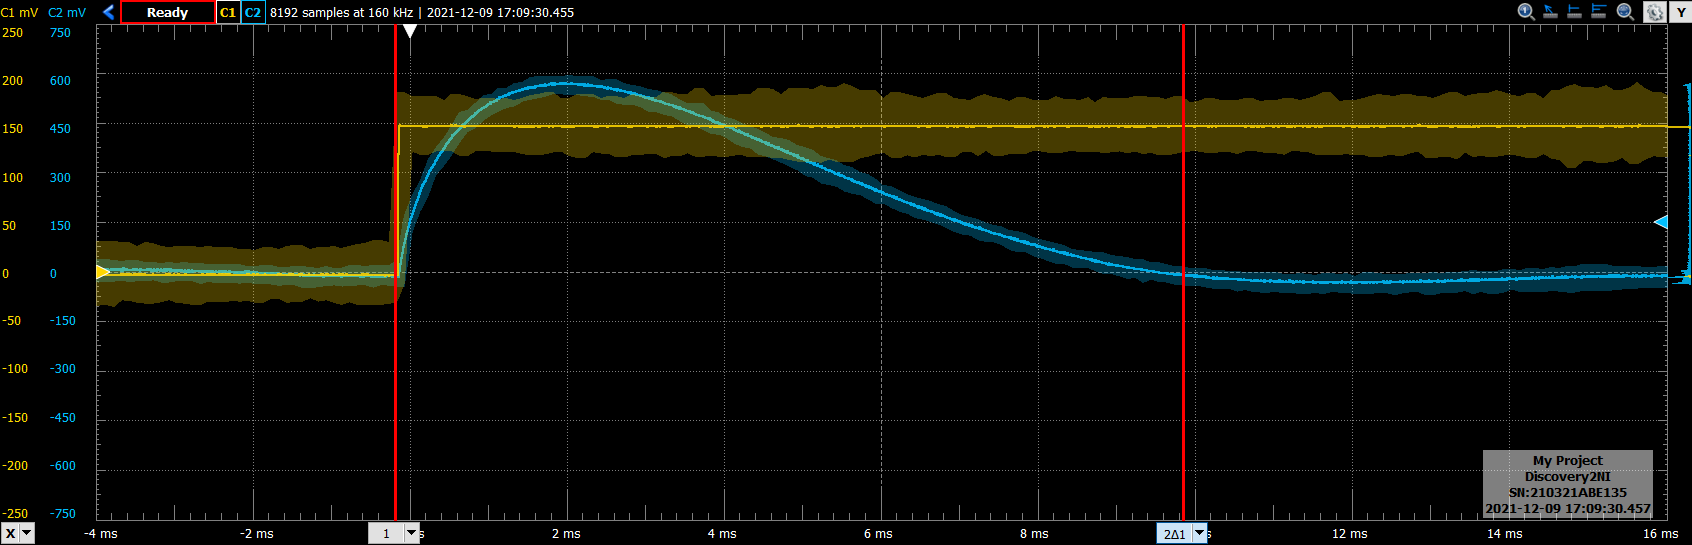
\includegraphics[scale=0.7]{7}
    \caption{Andamento del segnale error in blu, rispetto al segnale pilota del led di disturbo
    \label{fig: Draft1}}
\end{figure}
Tramite cursori si è poi preso il tempo con cui il segnale oscilla e lo abbiamo paragonato al tempo caratteristico del circuito integratore definito come $\tau = R_9C_1$.
\begin{table}[H]
\centering
\begin{tabular}{@{}lll@{}}
\toprule
$Resistenza Eq.$ & $Tempo C. misurato$ & $Tempo C. Atteso$\\
\midrule
$103.4 \pm 0.8 $ k$\ohm$ & $20.7 \pm 0.3$ ms  	& $ 21.4 \pm 0.9$ ms	\\
$92.8 \pm 0.8$ k$\ohm$ & $19.0 \pm 0.2$ ms 	& $ 19.2 \pm 0.8 $ ms	\\
$67.7 \pm 0.6$ k$\ohm$ & $15.3 \pm 0.2$ ms 	& $ 14.0 \pm 0.6 $ ms\\
$41.5 \pm 0.4$ k$\ohm$ & $10.2 \pm 0.1$ 	ms & $ 8.6 \pm 0.3 $ ms\\
$25.5 \pm 0.3$ k$\ohm$ & $7.78 \pm 0.05$ 	ms & $ 5.3 \pm 0.2 $ ms\\
$7.34 \pm0.06$ k$\ohm$ & $3.24 \pm 0.05$ 	ms & $ 1.52 \pm 0.06$ ms\\

\bottomrule
\end{tabular}
\caption{Misura dei tempi caratteristici delle oscillazioni del segnale di errore}
\end{table}
Nonostante le prime  2 o 3 misure risultino compatibili tra di loro, le altre si distaccano anche di molto dall'andamento previsto; si è notato inoltre come il tempo caratteristico misurato dipendesse anche dal valore di Set, parametro che non era presente nell'equazione di riferimento.
\subsection{Risposta ad una rampa}
Riportando il valore della resistenza equivalente al potenziometro a $100 k\ohm$ si è pilotato il driver led di disturbo con un'onda triangolare tra 0 e 150 mV a 10 Hz e nelle condizioni in cui il duty cycle fosse $10 \percent$ e $90 \percent$
\begin{figure}[H]
    \centering
	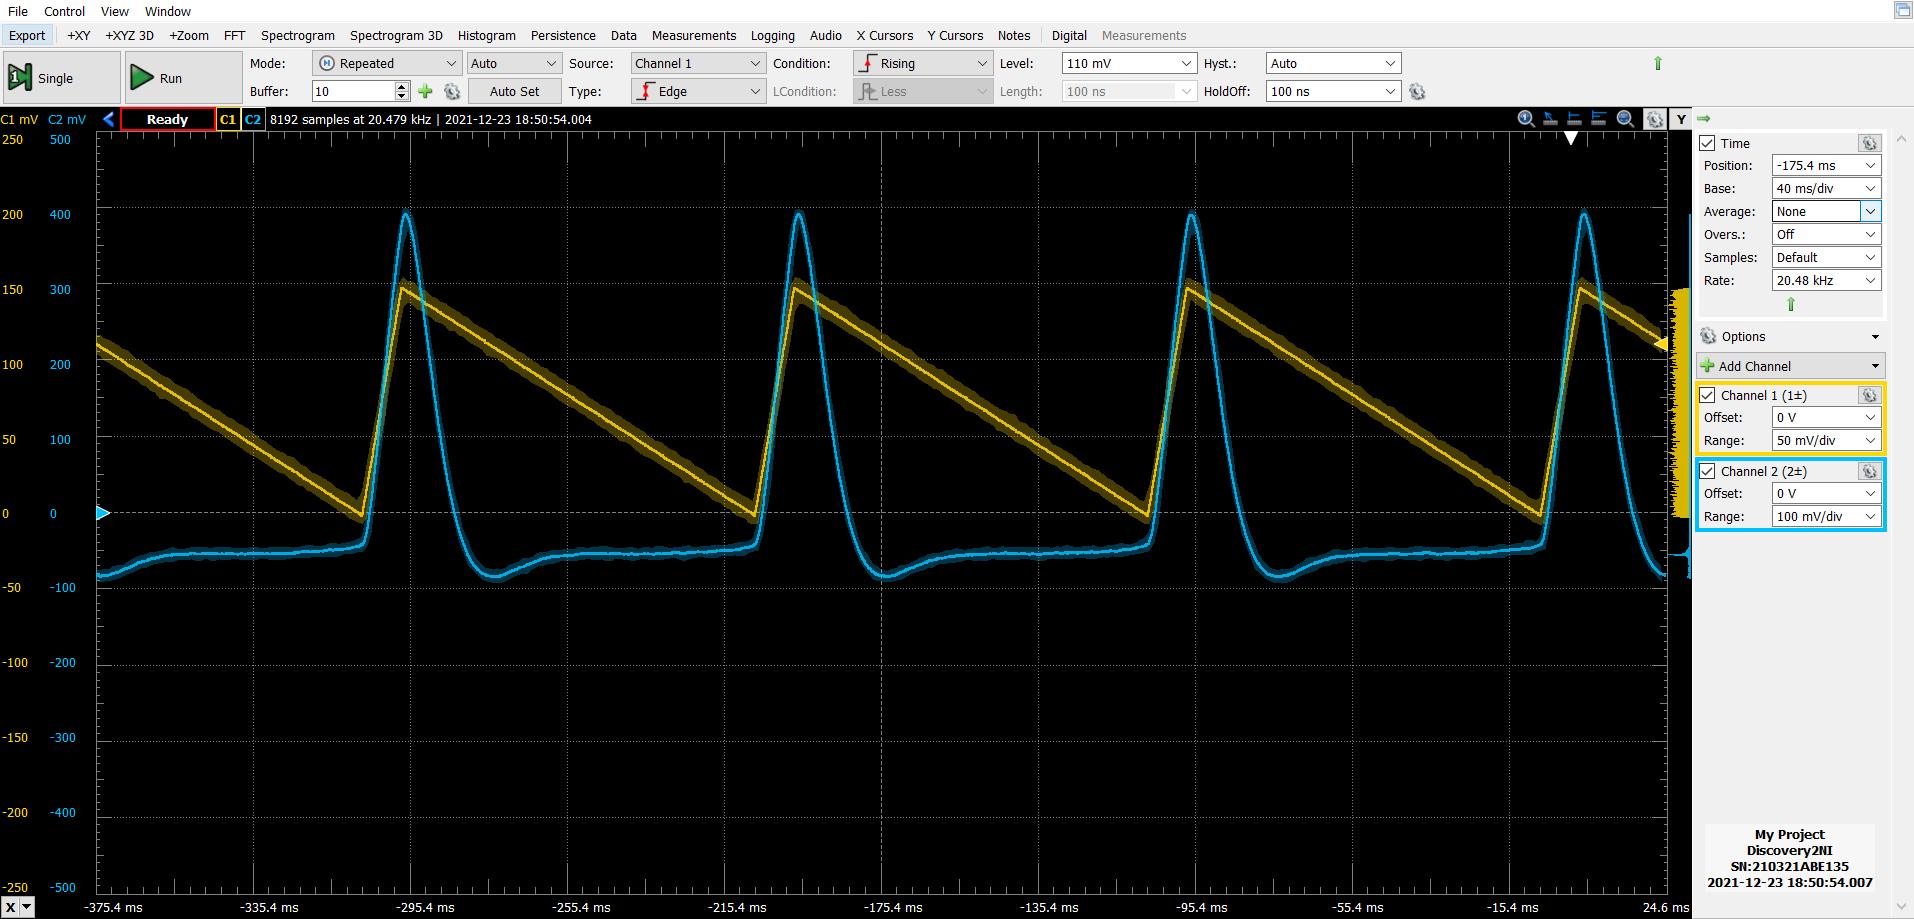
\includegraphics[scale=0.7]{8}
    \caption{grafico degli andamenti di error (rispetto a massa) in blu e del segnale in ingresso al led di disturbo (sempre rispetto a massa) in giallo pilotato con l'onda triangolare sopracitata con duty cycle $10 \percent$
    \label{fig: Draft1}}
\end{figure}

\begin{figure}[H]
    \centering
	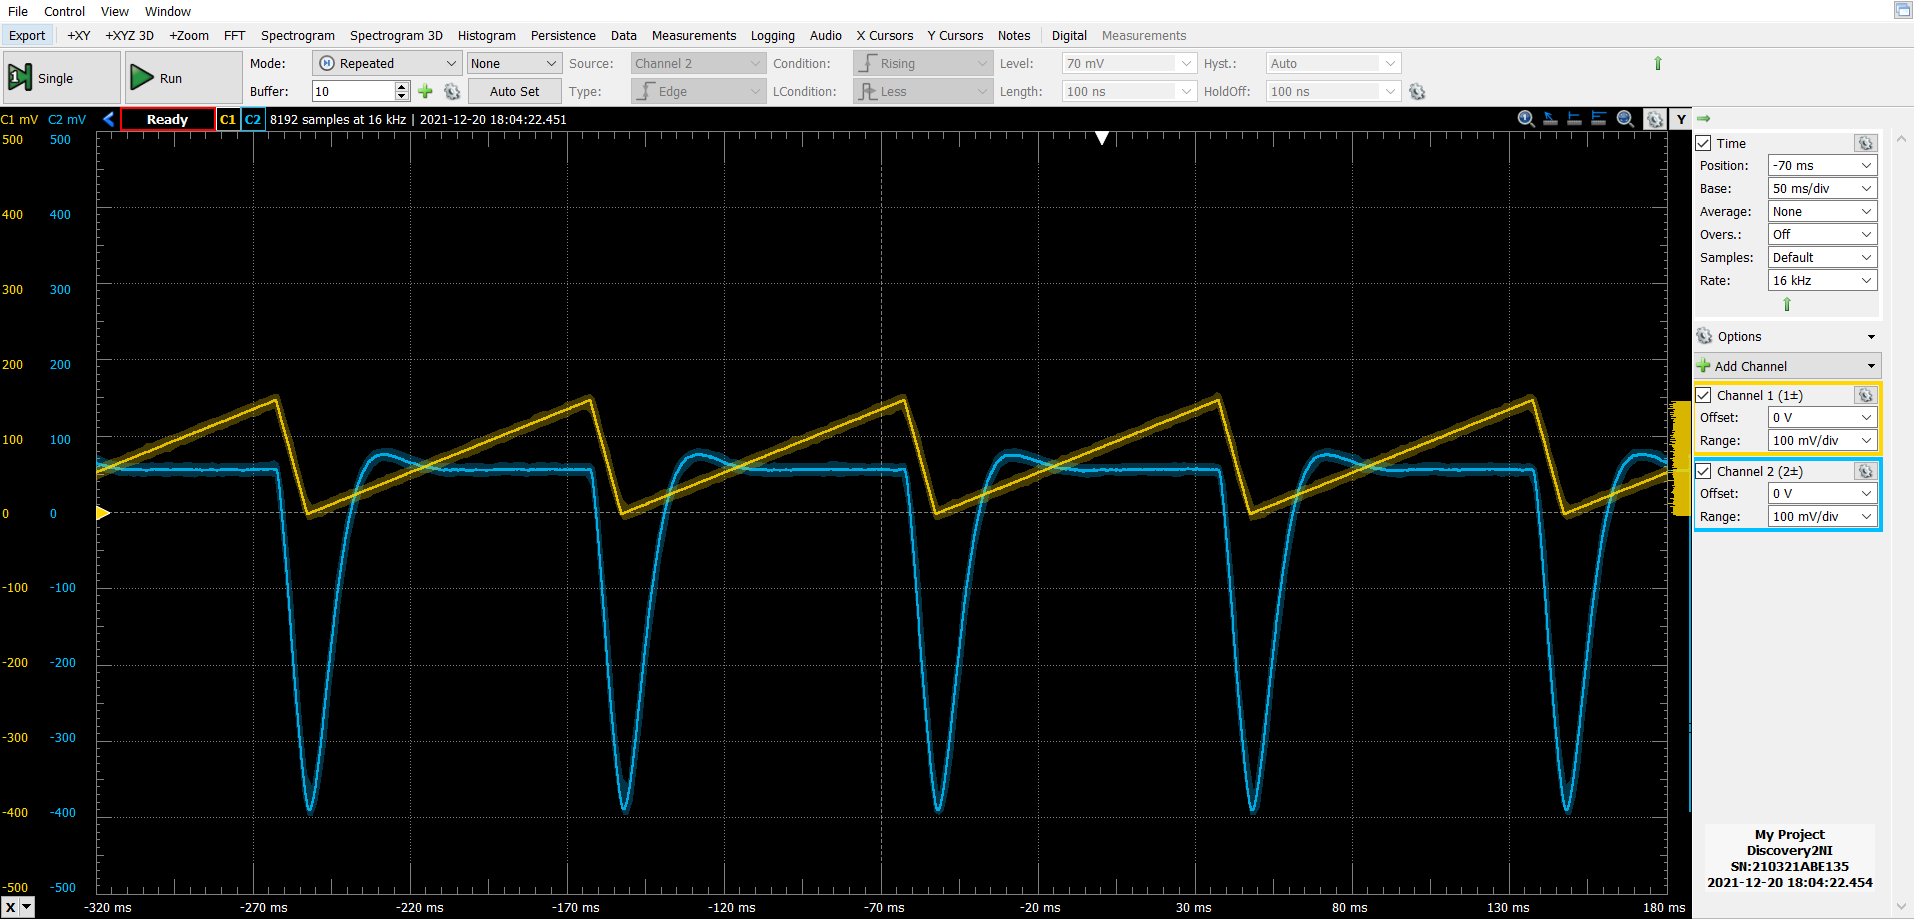
\includegraphics[scale=0.7]{8.1}
    \caption{grafico degli andamenti di error (rispetto a massa) in blu e del segnale in ingresso al led di disturbo (sempre rispetto a massa) in giallo pilotato con l'onda triangolare sopracitata con duty cycle $90 \percent$
    \label{fig: Draft1}}
\end{figure}
In questo caso il circuito di amplificazione dell'errore si comporta quasi come un derivatore: in fin dei conti è quello che ci si aspetta, dato che il controllo deve integrare il segnale di errore, per poter bilanciare il cambiamento di luce, c'è bisogno che anche l'uscita del controllo sia un'onda triangolare simmetrica a quella con cui pilotiamo il led di disturbo. Inoltre dato che il circuito integratore agisce in un tempo non trascurabile di fronte a dei cambiamenti,il segnale di errore non potrà mai essere nullo, infatti se lo fosse il controllore non produrrebbe alcun cambiamento, cosa che può sussistere solo nel caso in cui si abbia una luce di disturbo costante nel tempo.
\subsection{Risposta in frequenza}
\begin{figure}[H]
    \centering
	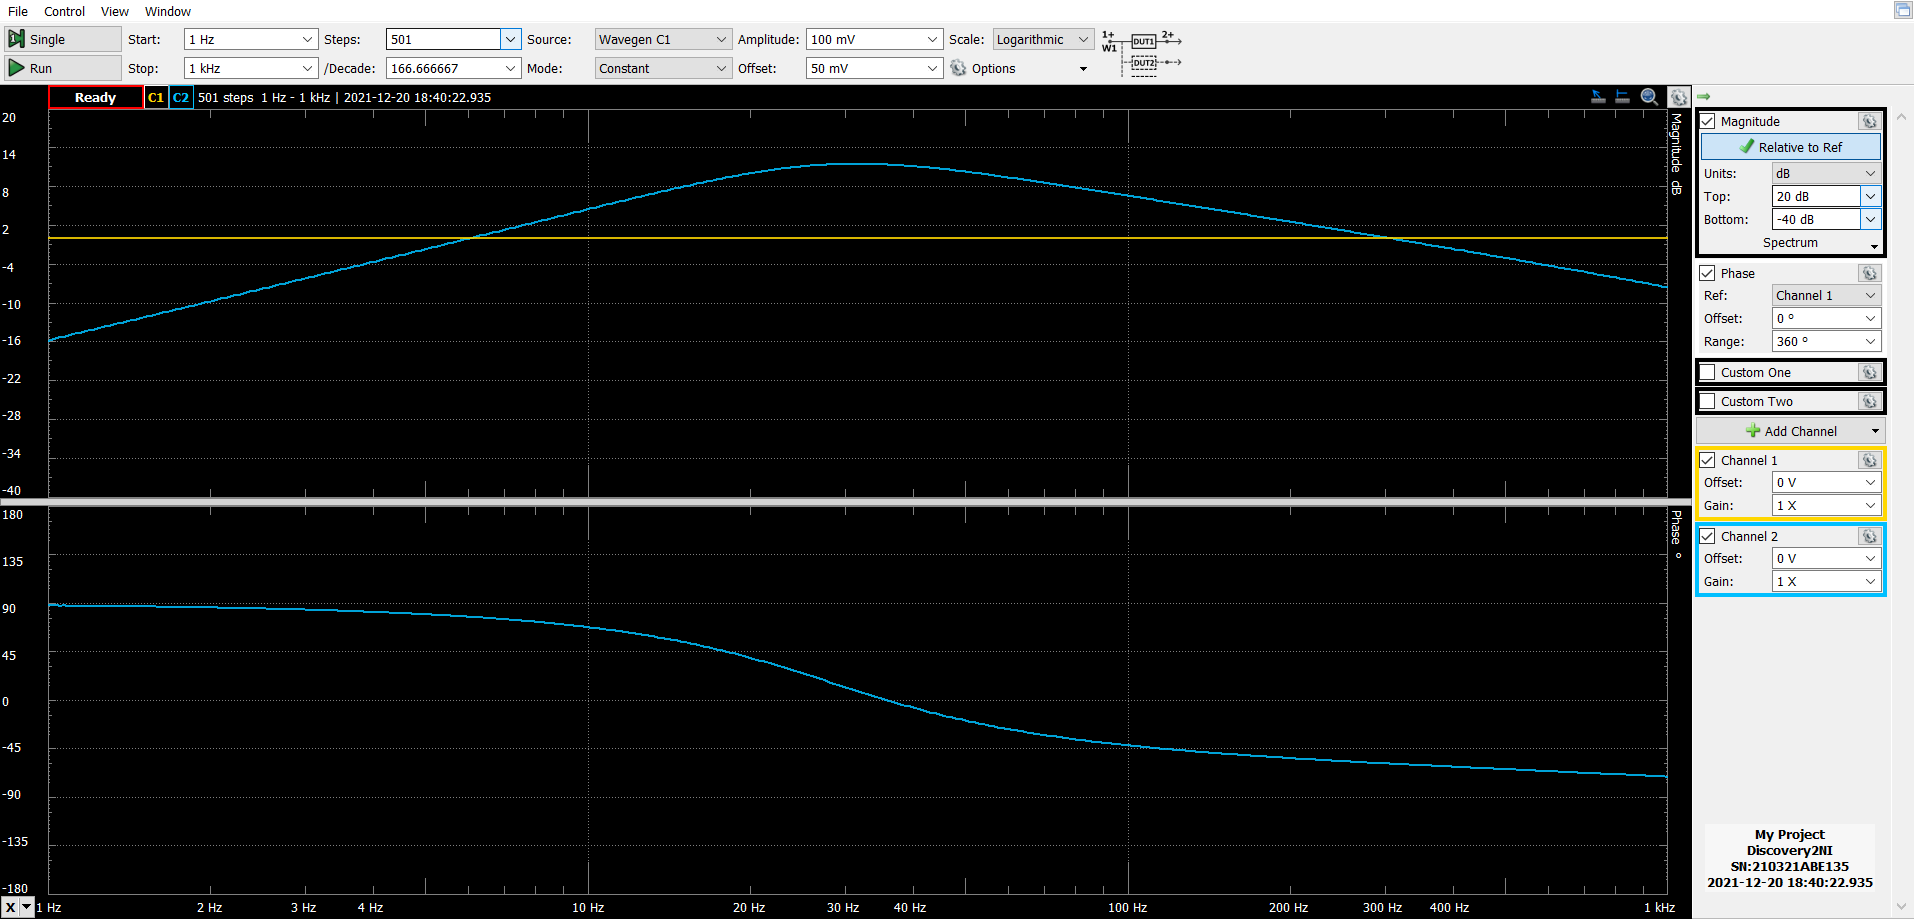
\includegraphics[scale=0.7]{103.4k}
    \caption{scan di network della funzione di trasferimento tra il generatore di disturbo e error con $R_9= 103.4 \pm 0.8 k\ohm$
    \label{fig: Draft1}}
\end{figure}
\begin{figure}[H]
    \centering
	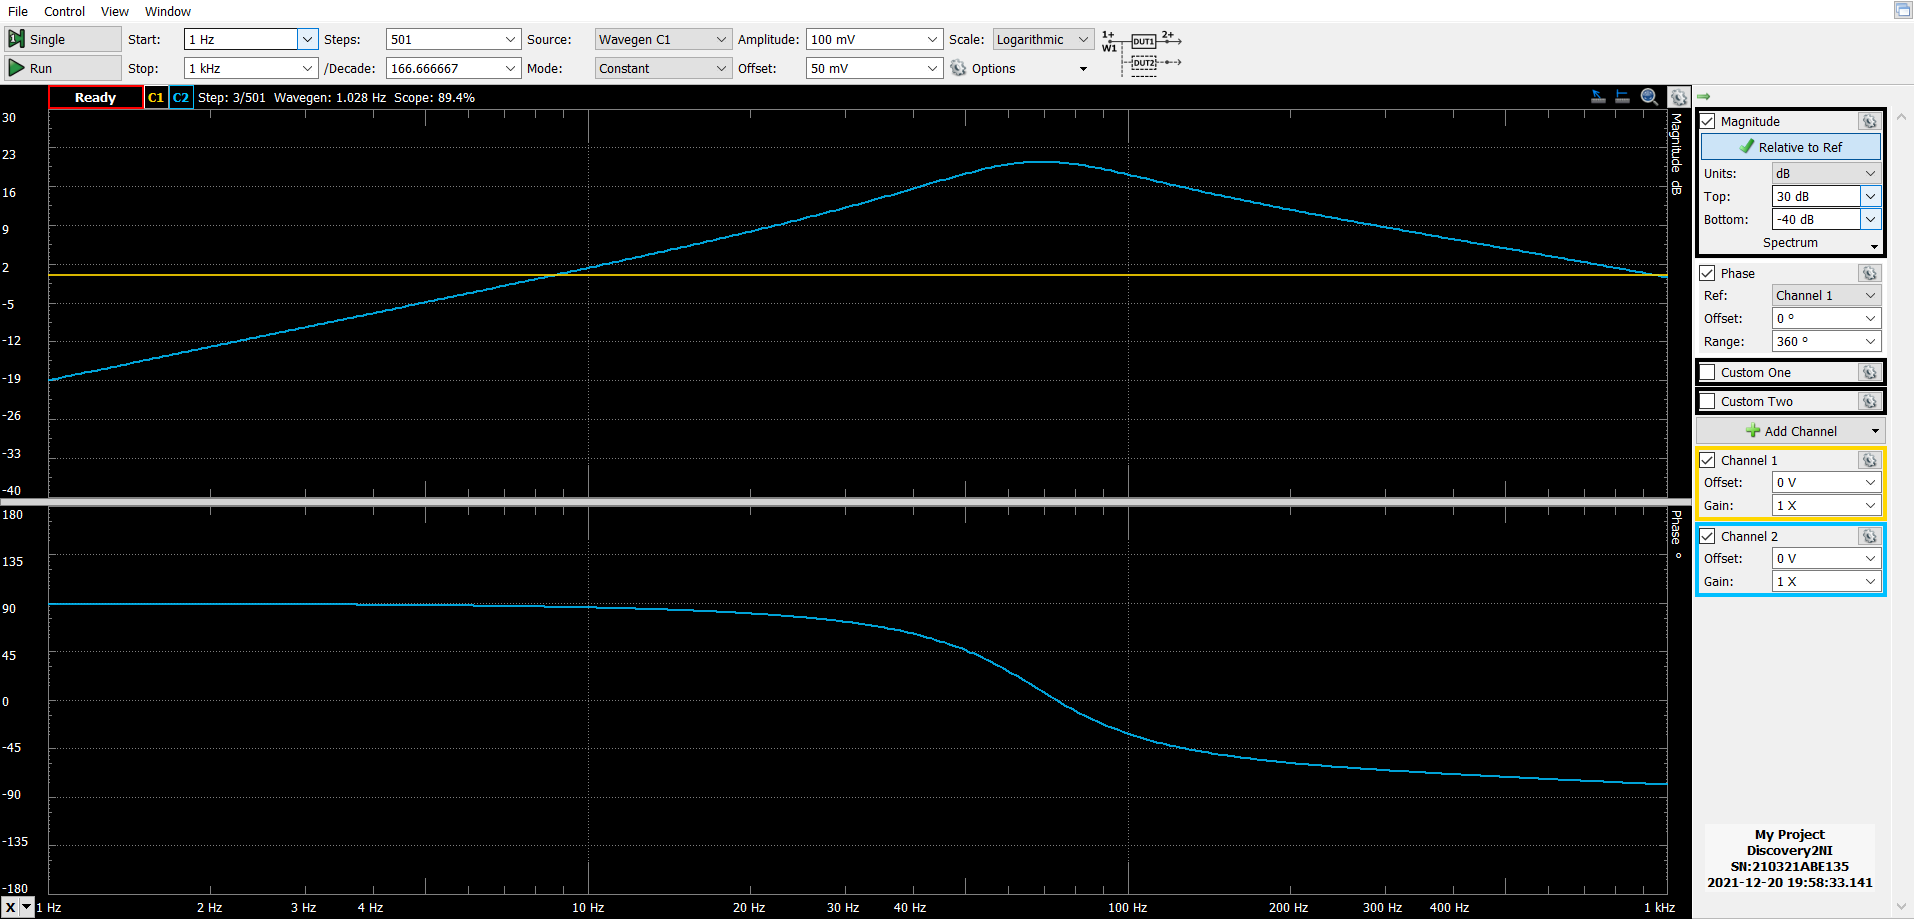
\includegraphics[scale=0.7]{76.1k}
    \caption{scan di network della funzione di trasferimento tra il generatore di disturbo e error con $R_9=76.1 \pm 0.6 k\ohm$
    \label{fig: Draft1}}
\end{figure}
\begin{figure}[H]
    \centering
	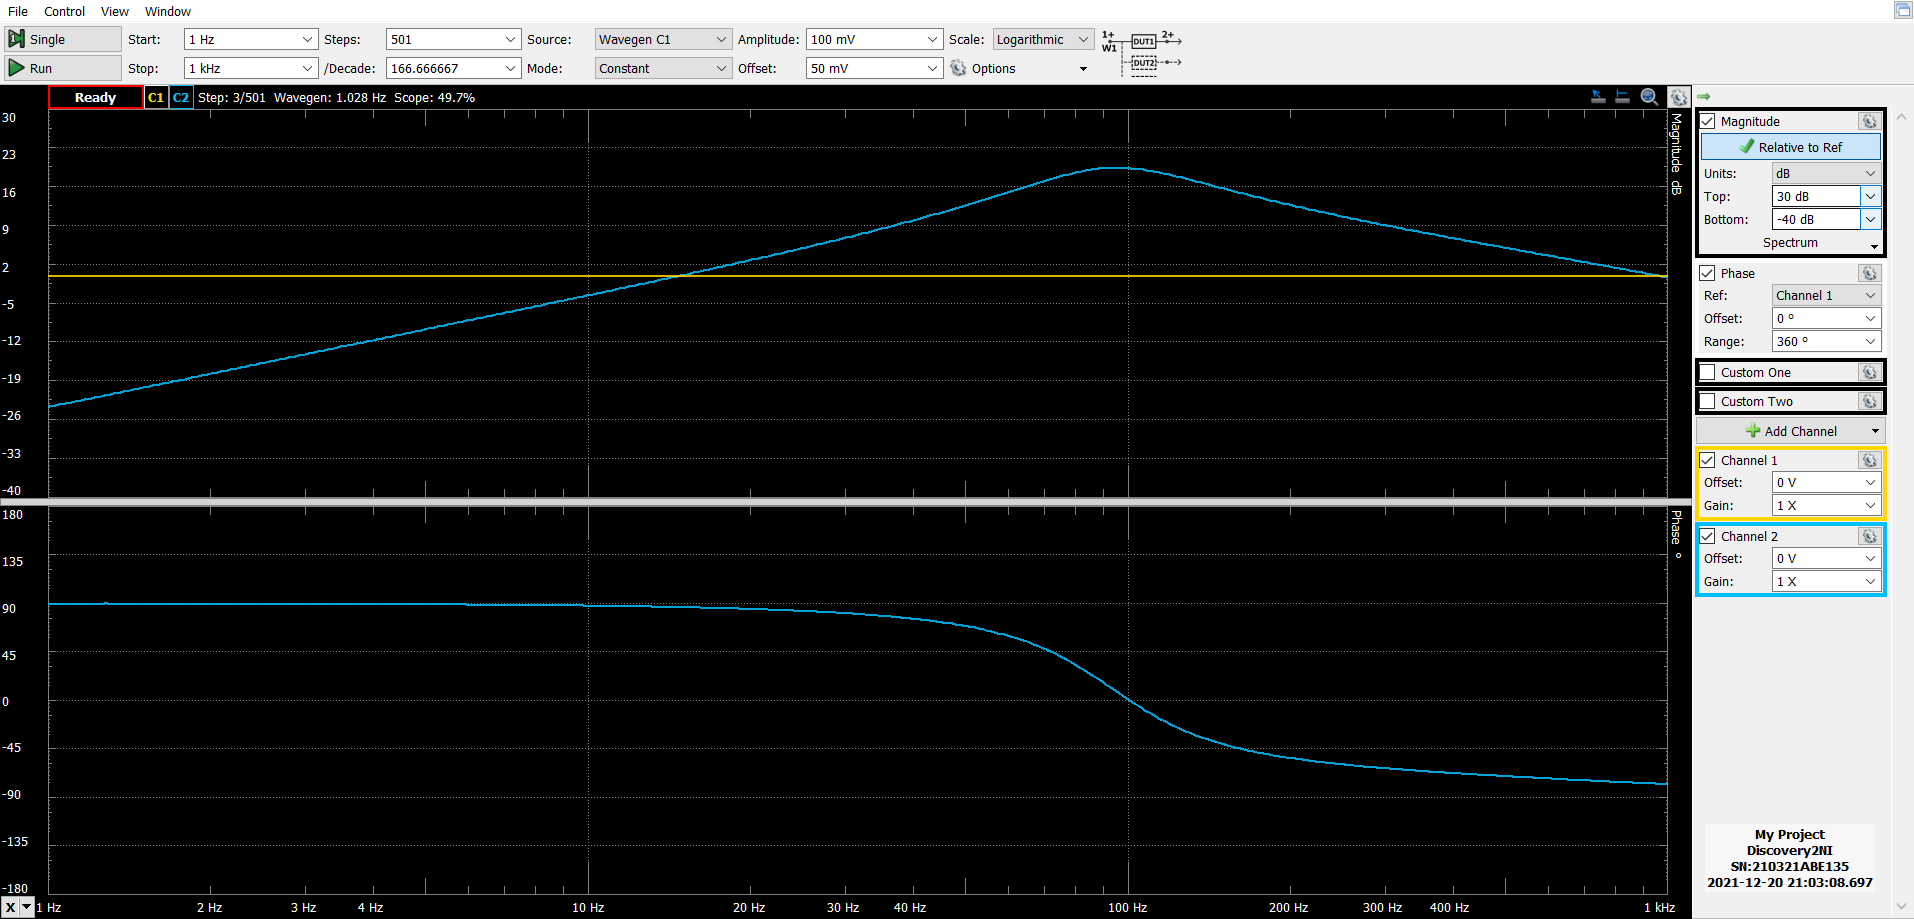
\includegraphics[scale=0.7]{43.9k}
    \caption{scan di network della funzione di trasferimento tra il generatore di disturbo e error con $R_9= 43.9 \pm 0.4 k\ohm$
    \label{fig: Draft1}}
\end{figure}
%=======================
\section{Controllo proporzionale}
Infine si è montato il circuito di controllo proporzionale al posto di quello integrale, scambiando il condensatore $C_1$ con una resistenza da$100 k\ohm$, secondo lo schema in figura.
\begin{figure}[H]
    \centering
	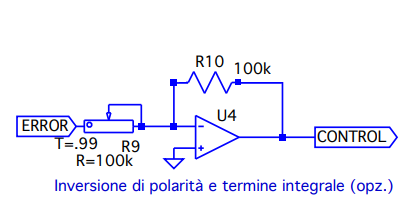
\includegraphics[scale=0.7]{controlgenprop}
    \caption{schema circuitale del controllore ad azione proporzionale.
    \label{fig: Draft1}}
\end{figure}
\subsection{Risposta ad un'onda quadra}
Come precedentemente fatto, dopo aver variato il potenziometro $R_9$ fino alla resistenza equivalente da $100 k\ohm$, abbiamo pilotato il driver led di disturbo con un'onda quadra tra 0 e 150 mV di 1Hz. Abbiamo quindi verificato la nuova situazione controllando i segnali prodotti da error, control e meas.
\begin{figure}[H]
    \centering
	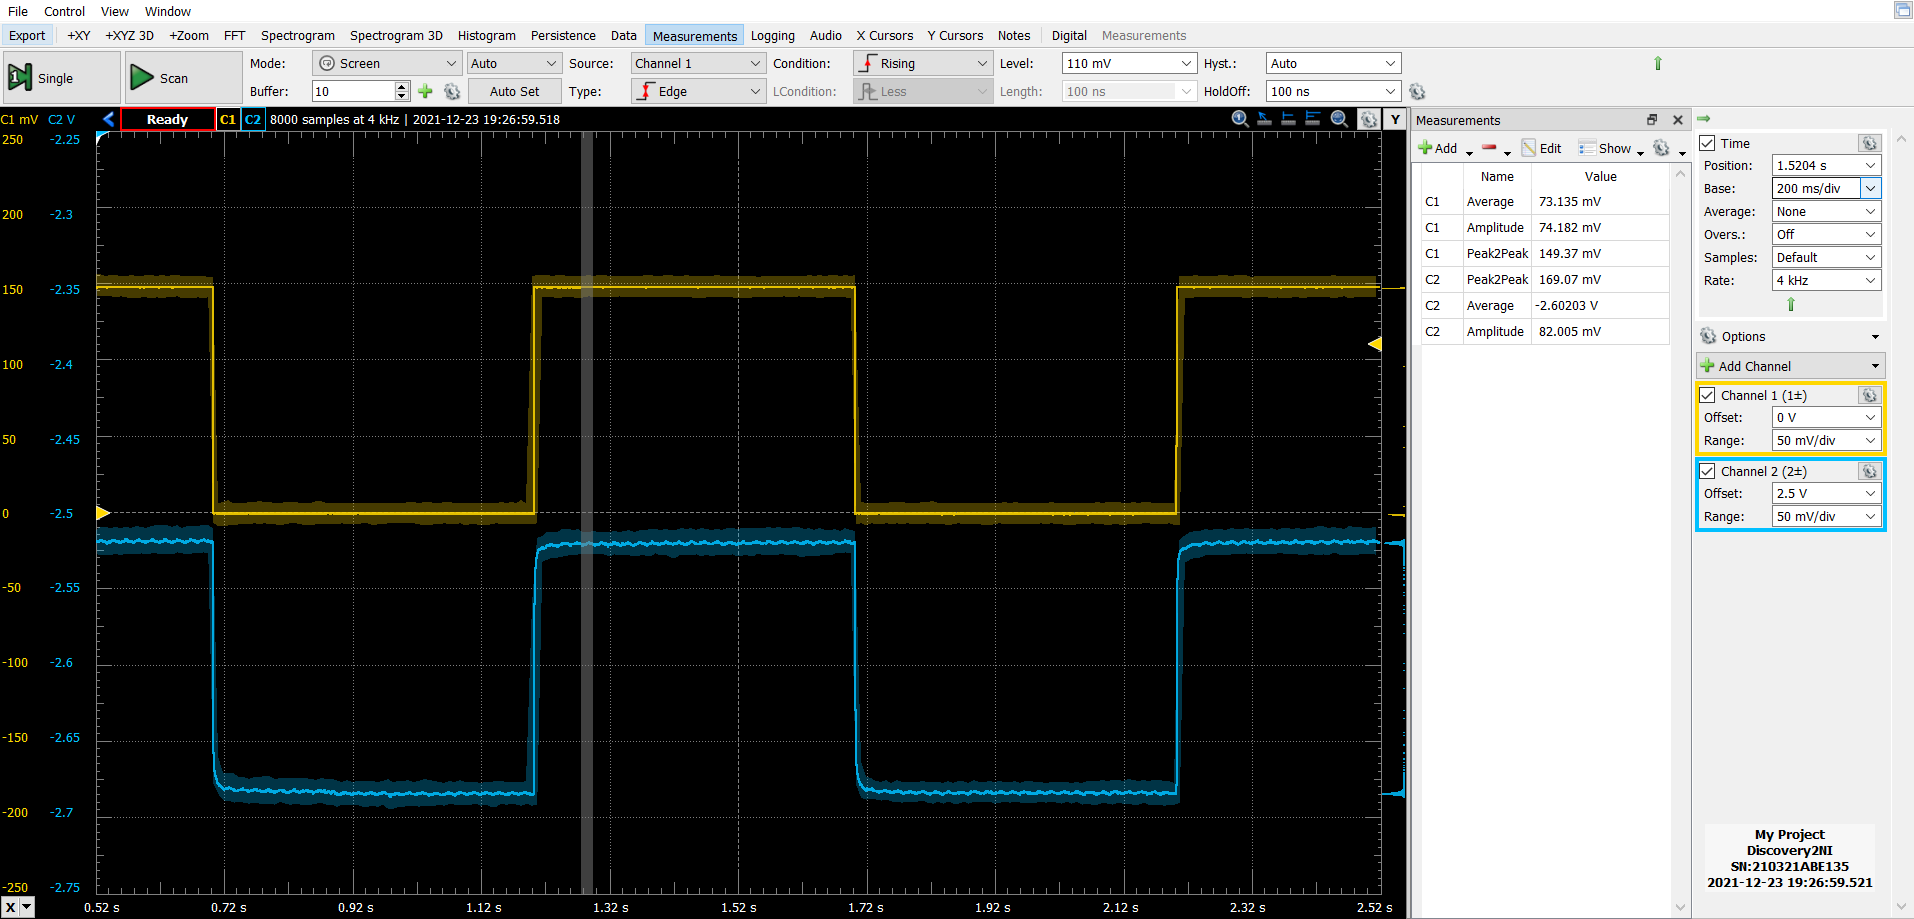
\includegraphics[scale=0.7]{proportional}
    \caption{grafico dei segnali error in blu e dell'onda pilota di disturbo in giallo.
    \label{fig: Draft1}}
\end{figure}
\begin{figure}[H]
    \centering
	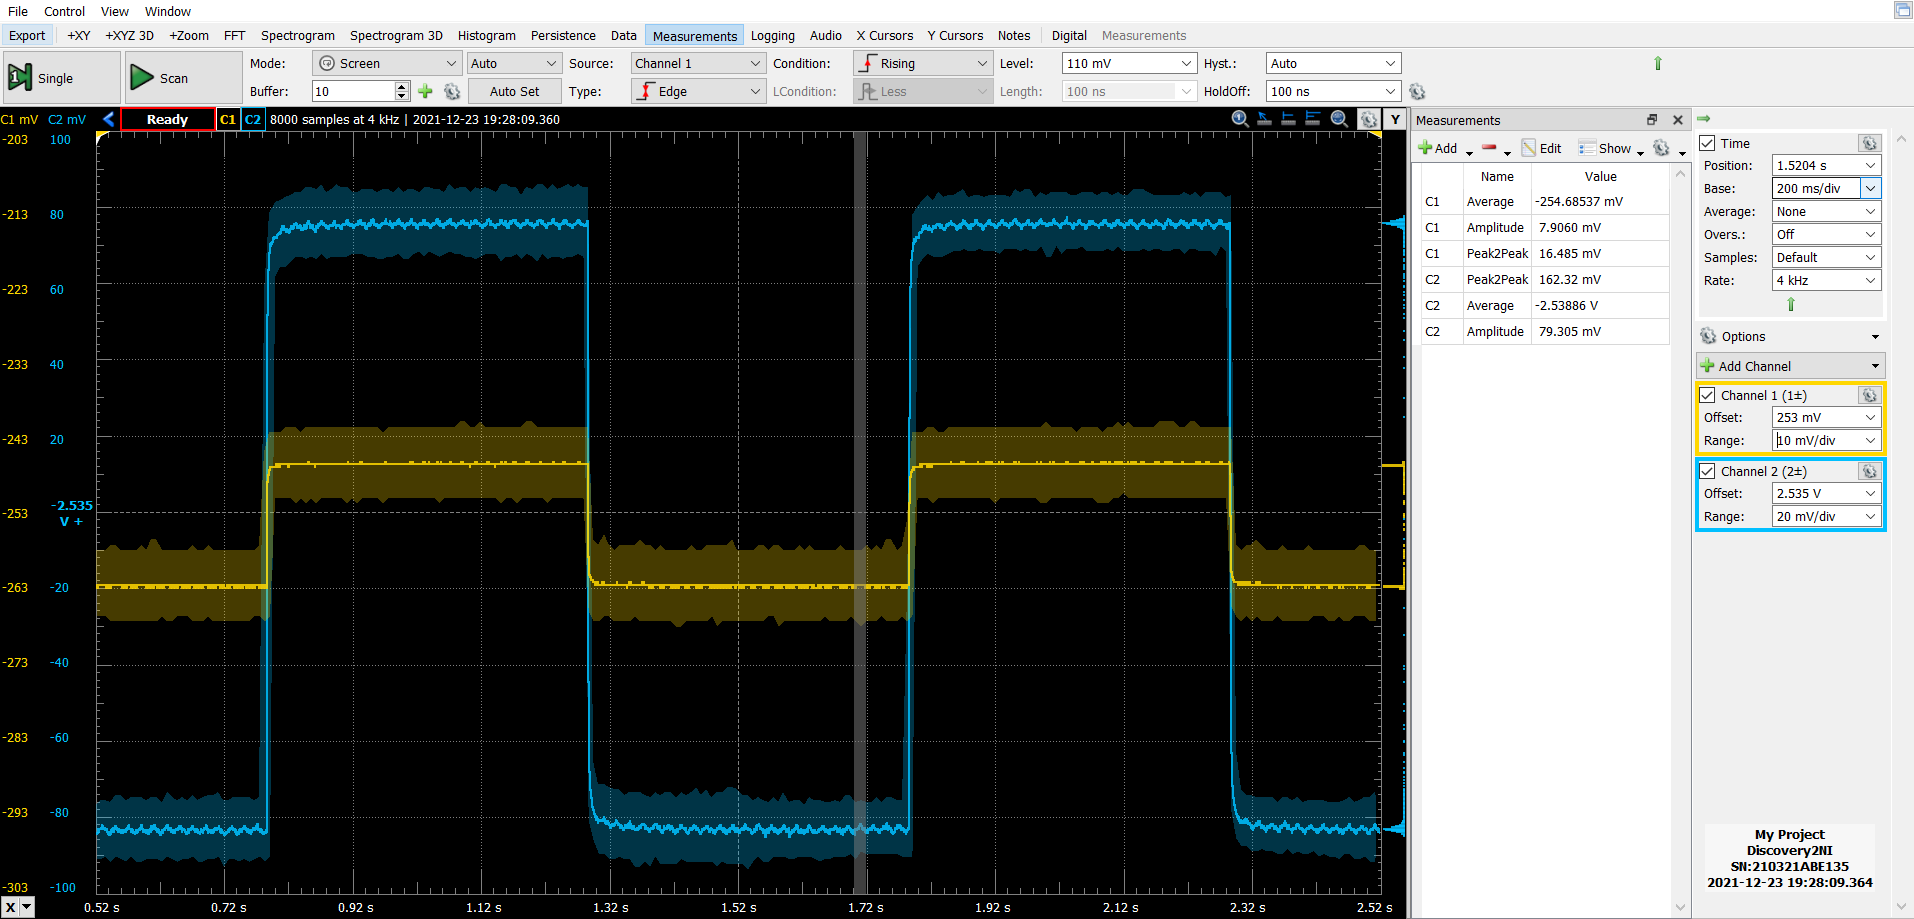
\includegraphics[scale=0.7]{proportional.meas}
    \caption{grafico dei segnali error in blu e di meas rispetto a set in giallo.
    \label{fig: Draft1}}
\end{figure}
\begin{figure}[H]
    \centering
	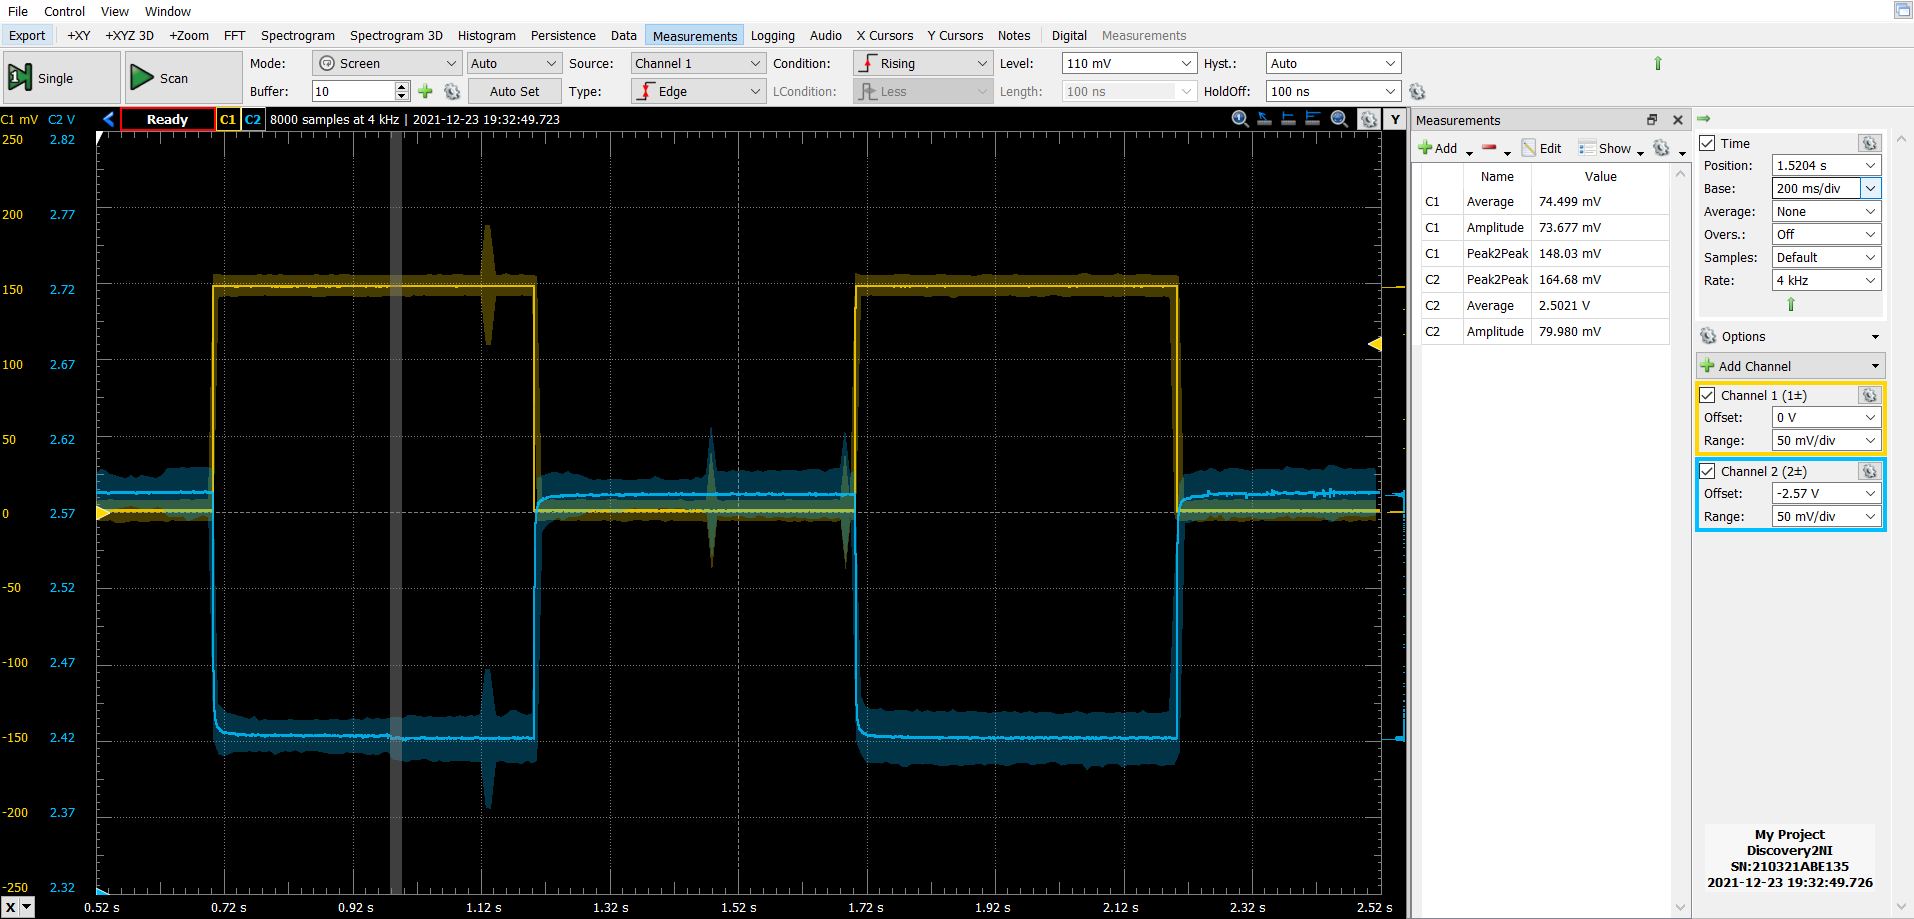
\includegraphics[scale=0.7]{proportional.control}
    \caption{grafico dei segnali control in blu e dell'onda pilota di disturbo in giallo.
    \label{fig: Draft1}}
\end{figure}
Come ci si aspettava il controllo proporzionale non mantiene meas invariato, dato che il circuito completo non è altro che una cascata di amplificatori, di cui il primo differenziale di guadagno $\approx 10$, e il secondo invertente di guadagno pari a $\frac{R_{10}}{R_9}$
%=======================
\section*{Conclusioni e commenti finali}


%=======================
\section*{Dichiarazione}
I firmatari di questa relazione dichiarano che il contenuto della relazione \`e
originale, con misure effettuate dai membri del gruppo, e che tutti i firmatari
hanno contribuito alla elaborazione della relazione stessa.


\end{document}
